\documentclass{ximera}

\author{Anna Davis} \title{MTH 140 Homework 8} 

\begin{document}

\begin{abstract}

\end{abstract}
\maketitle
 \textit{Certificate due: 10/19/2020 at 11:59 p.m.}
 
  \begin{center}
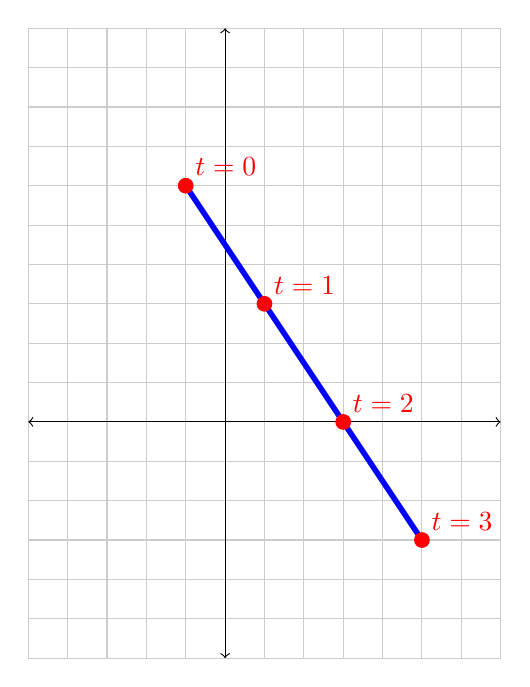
\begin{tikzpicture}[scale=0.5]
\draw[thin,gray!40] (-5,-6) grid (7,10);
  \draw[<->] (-5,0)--(7,0);
  \draw[<->] (0,-6)--(0,10);
  
\draw[line width=2pt,blue](-1,6)--(5,-3) ;

\fill[red] (-1,6) node[above right]{$t=0$} circle (0.2cm);
\fill[red] (1,3) node[above right]{$t=1$} circle (0.2cm);
\fill[red] (3,0) node[above right]{$t=2$} circle (0.2cm);
\fill[red] (5,-3) node[above right]{$t=3$} circle (0.2cm);
 
\end{tikzpicture}
\end{center}
 
\end{document}